\documentclass[10pt,report]{article}
\usepackage[utf8]{inputenc}
\usepackage[T1]{fontenc}
\usepackage{amsmath}
\usepackage{amssymb}
\usepackage{makeidx}
\usepackage{graphicx}
\usepackage{geometry}
\usepackage[colorlinks]{hyperref}
\usepackage[english]{babel}
\usepackage{siunitx}
\usepackage{booktabs}
\usepackage{minipage}
\usepackage{subcaption}
\title{Isotropic energy}
\author{Syed Ali Mohsin Bukhari}
\date{}
\begin{document}
	\maketitle
	\noindent\textbf{Determine the value for the isotropic energy of GRB120709A for different redshift values\footnote{z = [\num{1e-6}, 0.001, 0.01, 0.5, 0.1, 1, 2, 3]} in time-integrated as well as time-resolved analysis and see the evolution.}

%%%%%%%%%%%%%%%%%%%%%%%%%%%%%%%%%%%%%%%%%%%%%%%%%%%%%%%%%%%%%%%%%%%%%%%%%%%%%%%%%%%%%%%%%%%%%%%%%%%%

	\section{\SIrange{-0.128}{27.2}{\second}: SBPL model}
	\begin{minipage}[l]{0.48\textwidth}
		\centering
		\begin{tabular}{ccc}
			\toprule
			Redshift & E$_\text{peak}$ (1+z) [keV]& E$_\text{isotropic}$ [erg] \\
			\midrule
			0.1 & 395.935 & \num{5.032E46}\\
			0.5 & 539.711 & \num{1.351e48}\\
			1 & 720.435 & \num{5.327E48}\\
			2 & 1081.974 & \num{1.858e49}\\
			3 & 1438.839 & \num{3.556E48}\\
			4 & 1803.007 & \num{5.443E49}\\
			5 & 2161.165 & \num{7.407E49}\\
			6 & 2522.745 & \num{9.390E49}\\
			7 & 2884.922 & \num{1.137E50}\\
			8 & 3243.158 & \num{1.332E50}\\
			9 & 3606.052 & \num{1.523E50}\\
			10 & 3966.159 & \num{1.710E50}\\
			\bottomrule
		\end{tabular}
	\end{minipage}
	\hfill
	\begin{minipage}[r]{0.48\textwidth}
%		\vspace{25px}
		\centering
		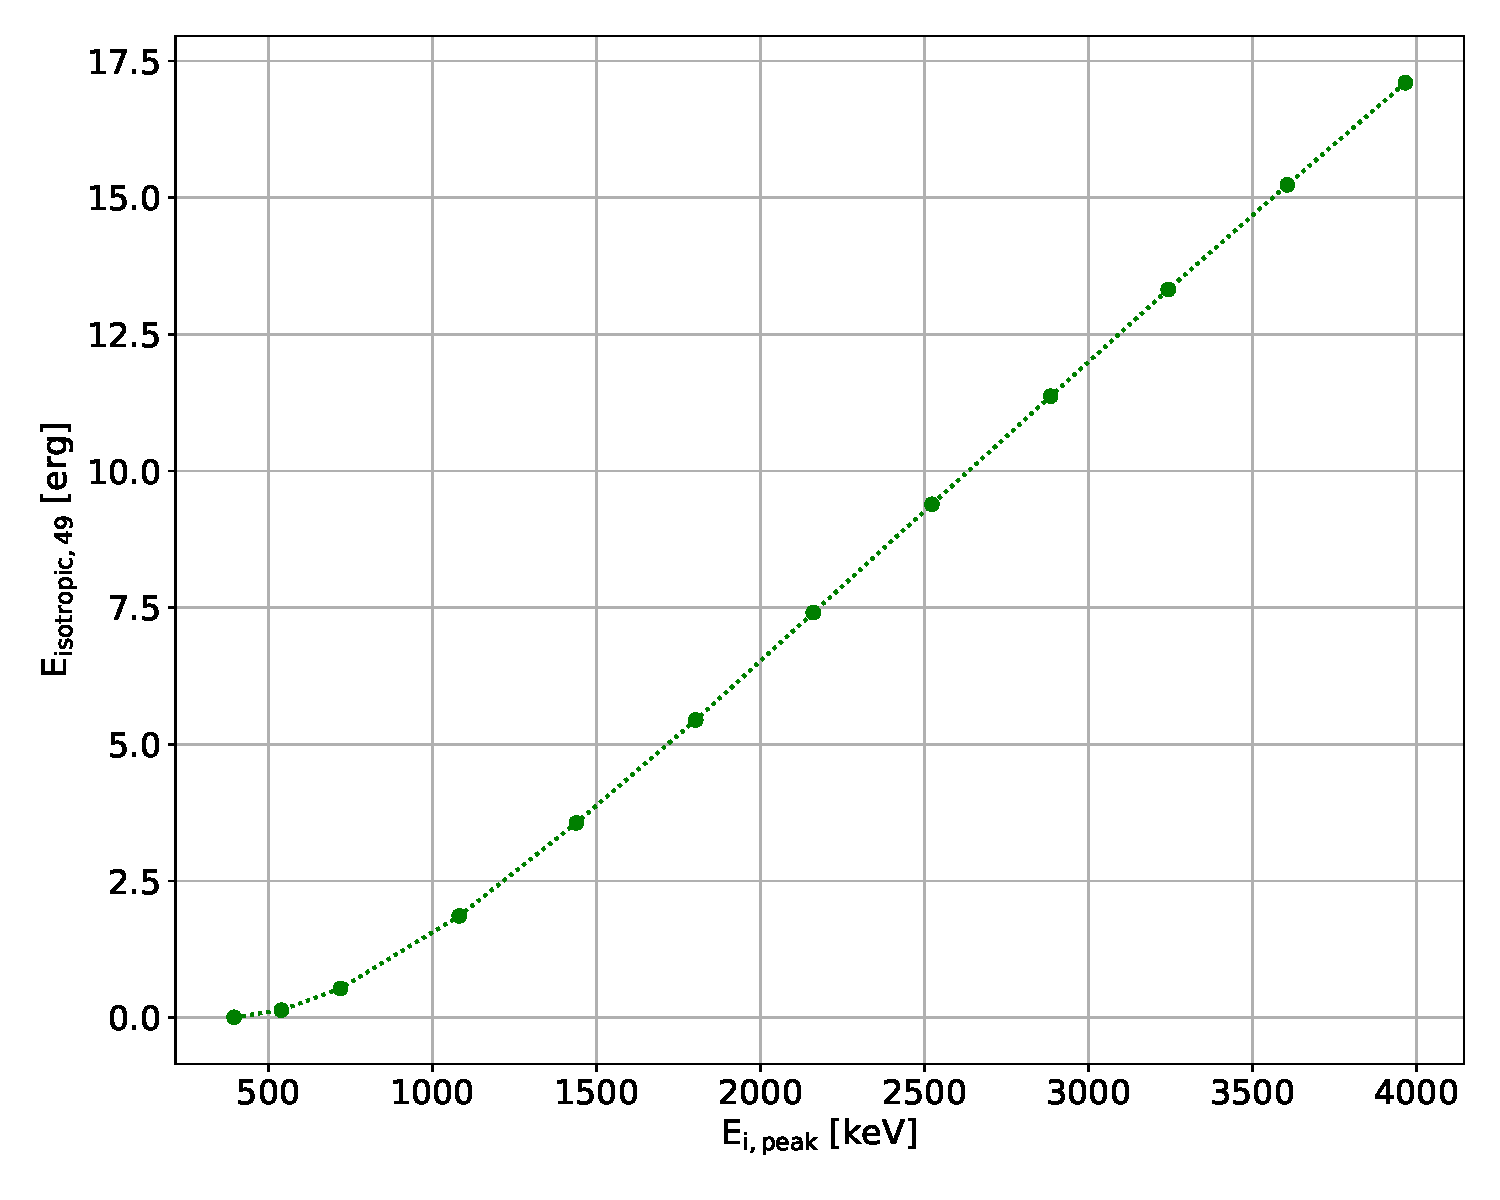
\includegraphics[width=\textwidth]{../TI/Ep0__eipeak_eisotropic}
%		\captionof*{figure}{}
	\end{minipage}%

%%%%%%%%%%%%%%%%%%%%%%%%%%%%%%%%%%%%%%%%%%%%%%%%%%%%%%%%%%%%%%%%%%%%%%%%%%%%%%%%%%%%%%%%%%%%%%%%%%%%

	\section{\SIrange{-0.128}{3.648}{\second}: SBPL model}
	\begin{minipage}[l]{0.48\textwidth}
		\centering
		\begin{tabular}{ccc}
			\toprule
			Redshift & E$_\text{peak}$ (1+z) [keV]& E$_\text{isotropic}$ [erg] \\
			\midrule
			0.1 & 492.432 & \num{1.322E46}\\
			0.5 & 670.313 & \num{3.491E47}\\
			1 & 897.052 & \num{1.352E48}\\
			2 & 1345.772 & \num{4.595E48}\\
			3 & 1795.498 & \num{8.636E48}\\
			4 & 2240.728 & \num{1.297E49}\\
			5 & 2689.516 & \num{1.739E49}\\
			6 & 3144.252 & \num{2.178E49}\\
			7 & 3582.959 & \num{2.606E49}\\
			8 & 4037.448 & \num{3.020E49}\\
			9 & 4480.831 & \num{3.418E49}\\
			10 & 4925.668 & \num{3.800E49}\\
			\bottomrule
		\end{tabular}
	\end{minipage}
	\hfill
	\begin{minipage}[r]{0.48\textwidth}
%		\vspace{25px}
		\centering
		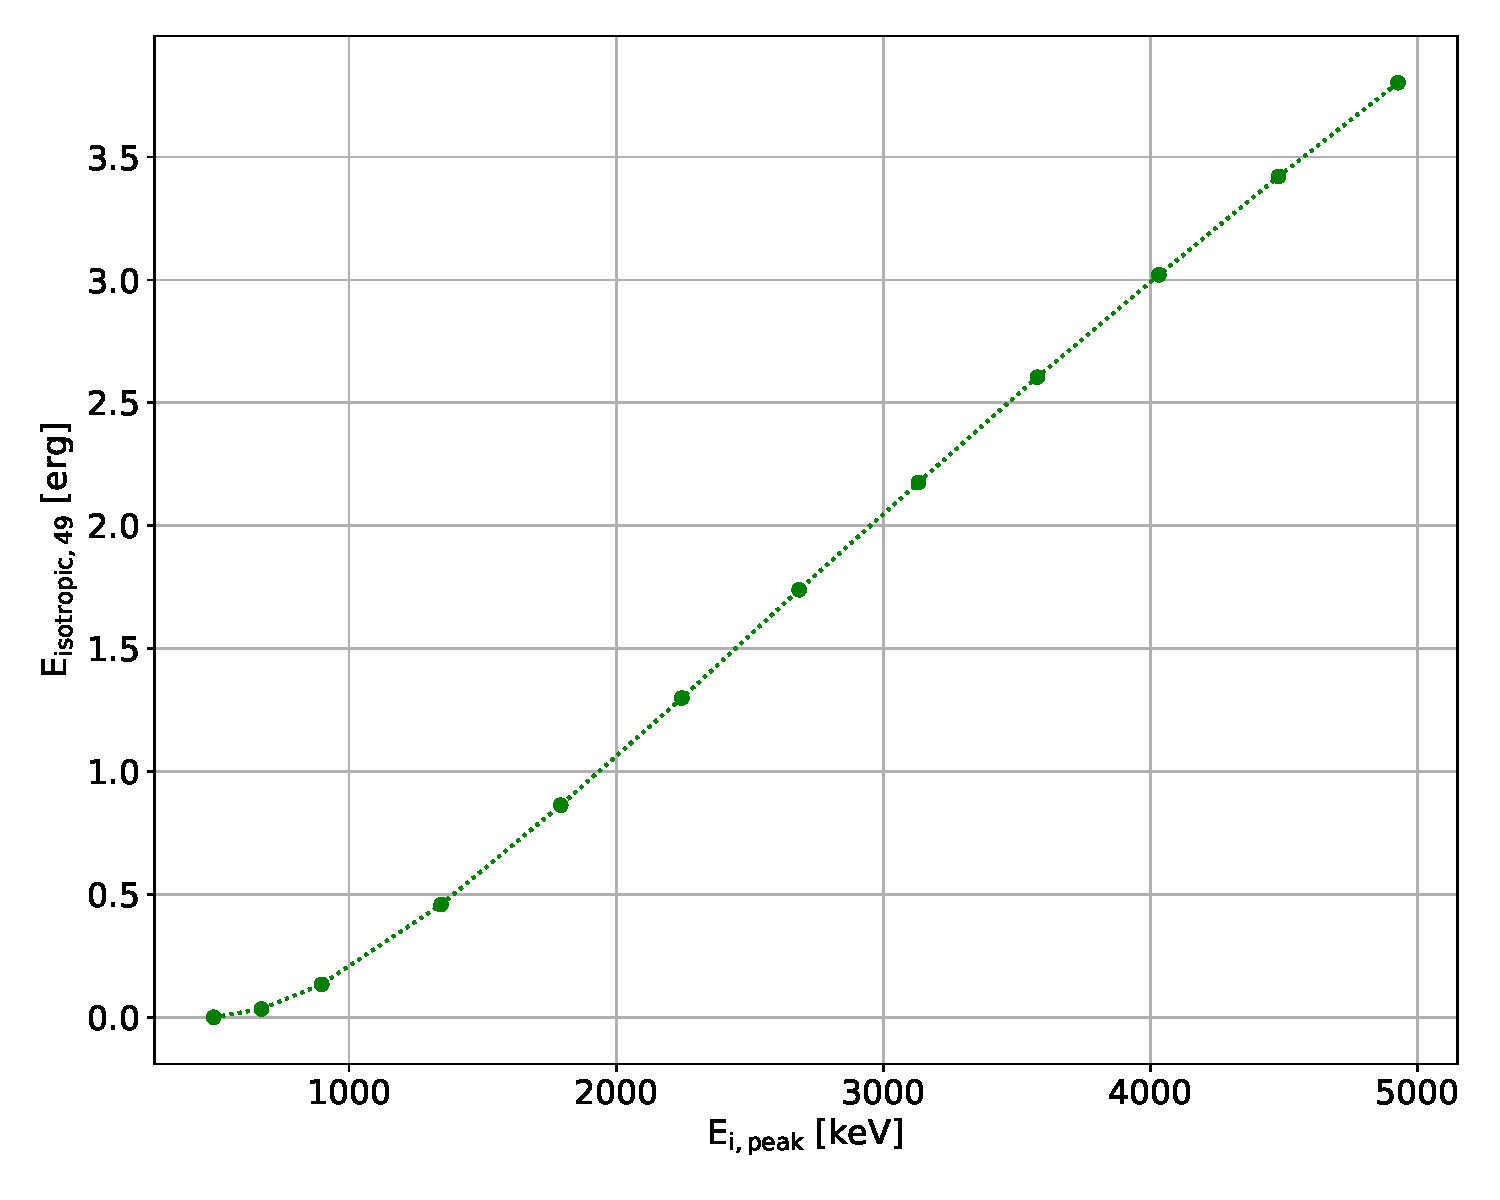
\includegraphics[width=\textwidth]{../ep1/Ep1__eipeak_eisotropic}
%		\captionof*{figure}{}
	\end{minipage}%

%%%%%%%%%%%%%%%%%%%%%%%%%%%%%%%%%%%%%%%%%%%%%%%%%%%%%%%%%%%%%%%%%%%%%%%%%%%%%%%%%%%%%%%%%%%%%%%%%%%%

	\section{\SIrange{10.432}{15.232}{\second}: Band model}
	\begin{minipage}[l]{0.48\textwidth}
		\centering
		\begin{tabular}{ccc}
			\toprule
			Redshift & E$_\text{peak}$ (1+z) [keV]& E$_\text{isotropic}$ [erg] \\
			\midrule
			0.1 & 492.681 & \num{9.024E45}\\
			0.5 & 671.647 & \num{2.425E47}\\
			1 & 893.492 & \num{9.541E47}\\
			2 & 1342.397 & \num{3.328E48}\\
			3 & 1789.708 & \num{6.377E48}\\
			4 & 2238.716 & \num{9.748E48}\\
			5 & 2690.130 & \num{1.324E49}\\
			6 & 3134.167 & \num{1.678E49}\\
			7 & 3587.862 & \num{2.030E49}\\
			8 & 4021.573 & \num{2.374E49}\\
			9 & 4474.865 & \num{2.713E49}\\
			10 & 4928.026 & \num{3.041E49}\\
			\bottomrule
		\end{tabular}
	\end{minipage}
	\hfill
	\begin{minipage}[r]{0.48\textwidth}
		\centering
		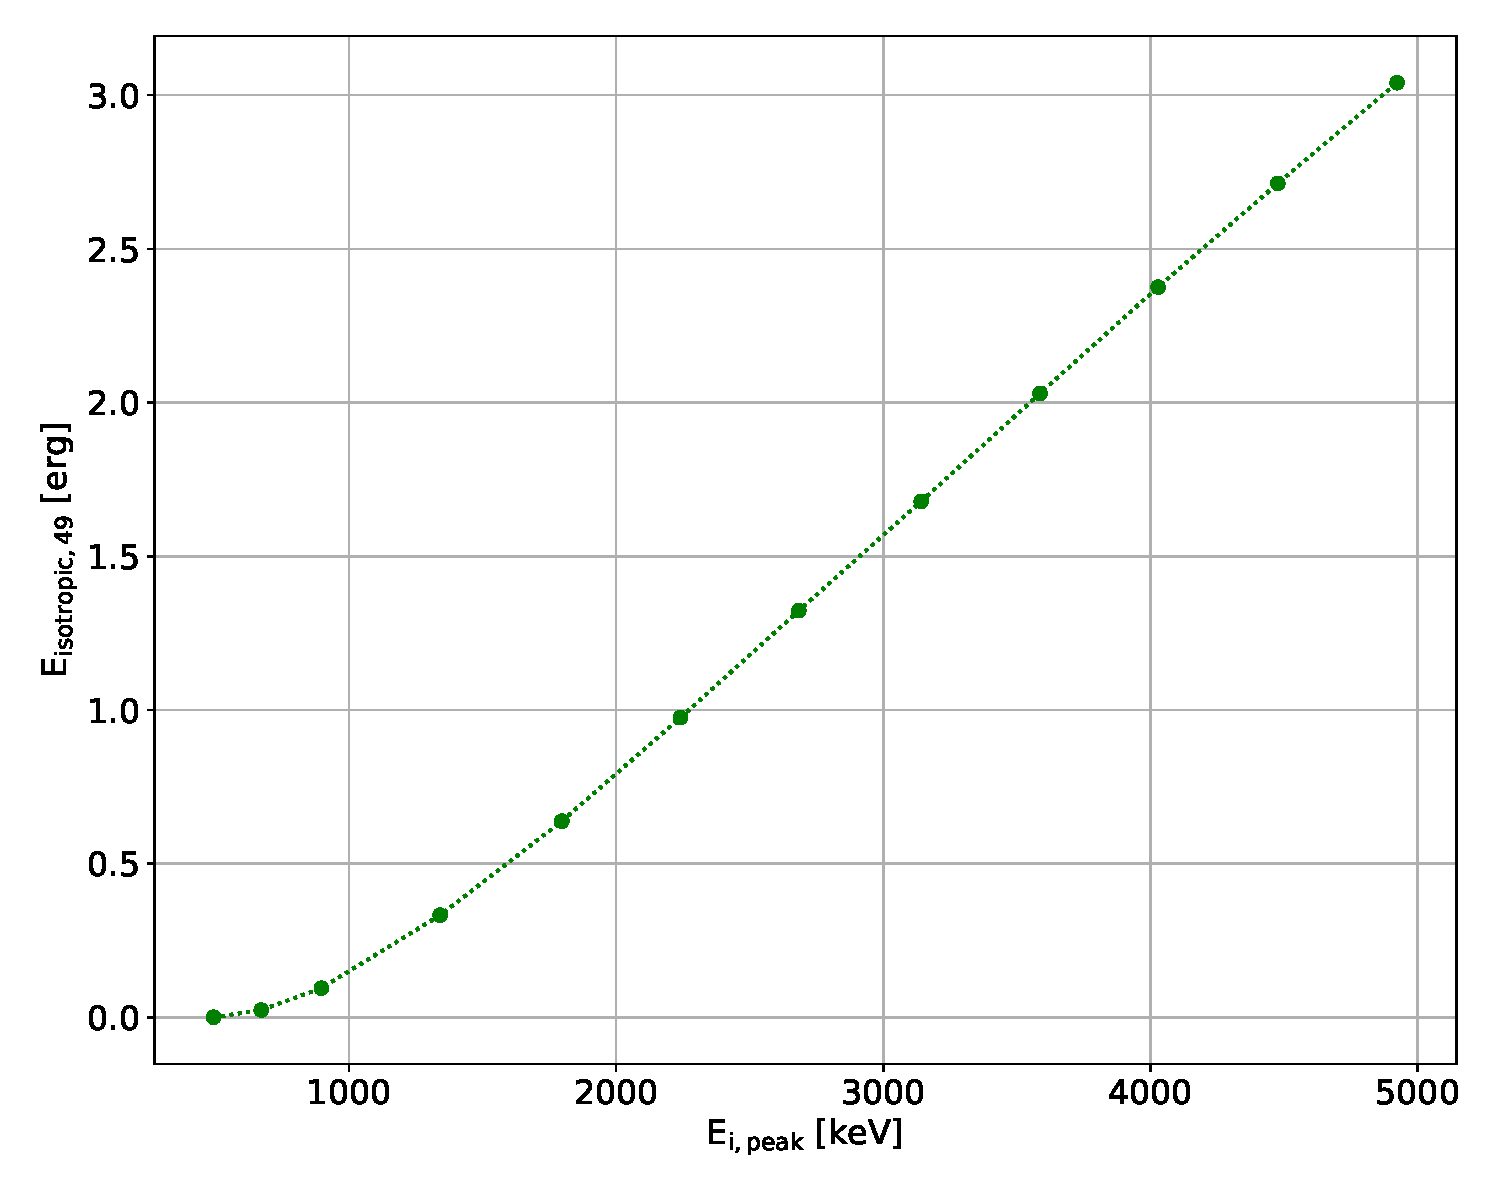
\includegraphics[width=\textwidth]{../ep2/Ep2__eipeak_eisotropic}%
%		\captionof{figure}{}
	\end{minipage}%

%%%%%%%%%%%%%%%%%%%%%%%%%%%%%%%%%%%%%%%%%%%%%%%%%%%%%%%%%%%%%%%%%%%%%%%%%%%%%%%%%%%%%%%%%%%%%%%%%%%%

	\section{\SIrange{21.184}{24.32}{\second}: CPL model}
	\begin{minipage}[l]{0.48\textwidth}
		\centering
		\begin{tabular}{ccc}
			\toprule
			Redshift & E$_\text{peak}$ (1+z) [keV]& E$_\text{isotropic}$ [erg] \\
			\midrule
			0.1 & 272.781 & \num{9.053E45}\\
			0.5 & 371.869 & \num{2.493E47}\\
			1 & 495.757 & \num{1.009E48}\\
			2 & 743.185 & \num{3.696E48}\\
			3 & 990.848 & \num{7.395E48}\\
			4 & 1237.845 & \num{1.173E49}\\
			5 & 1487.058 & \num{1.654E49}\\
			6 & 1733.886 & \num{2.165E49}\\
			7 & 1983.771 & \num{2.702E49}\\
			8 & 2231.076 & \num{3.251E49}\\
			9 & 2477.618 & \num{3.807E49}\\
			10 & 2725.357 & \num{4.370E49}\\
			\bottomrule
		\end{tabular}
	\end{minipage}
	\hfill
	\begin{minipage}[r]{0.48\textwidth}
		\centering
		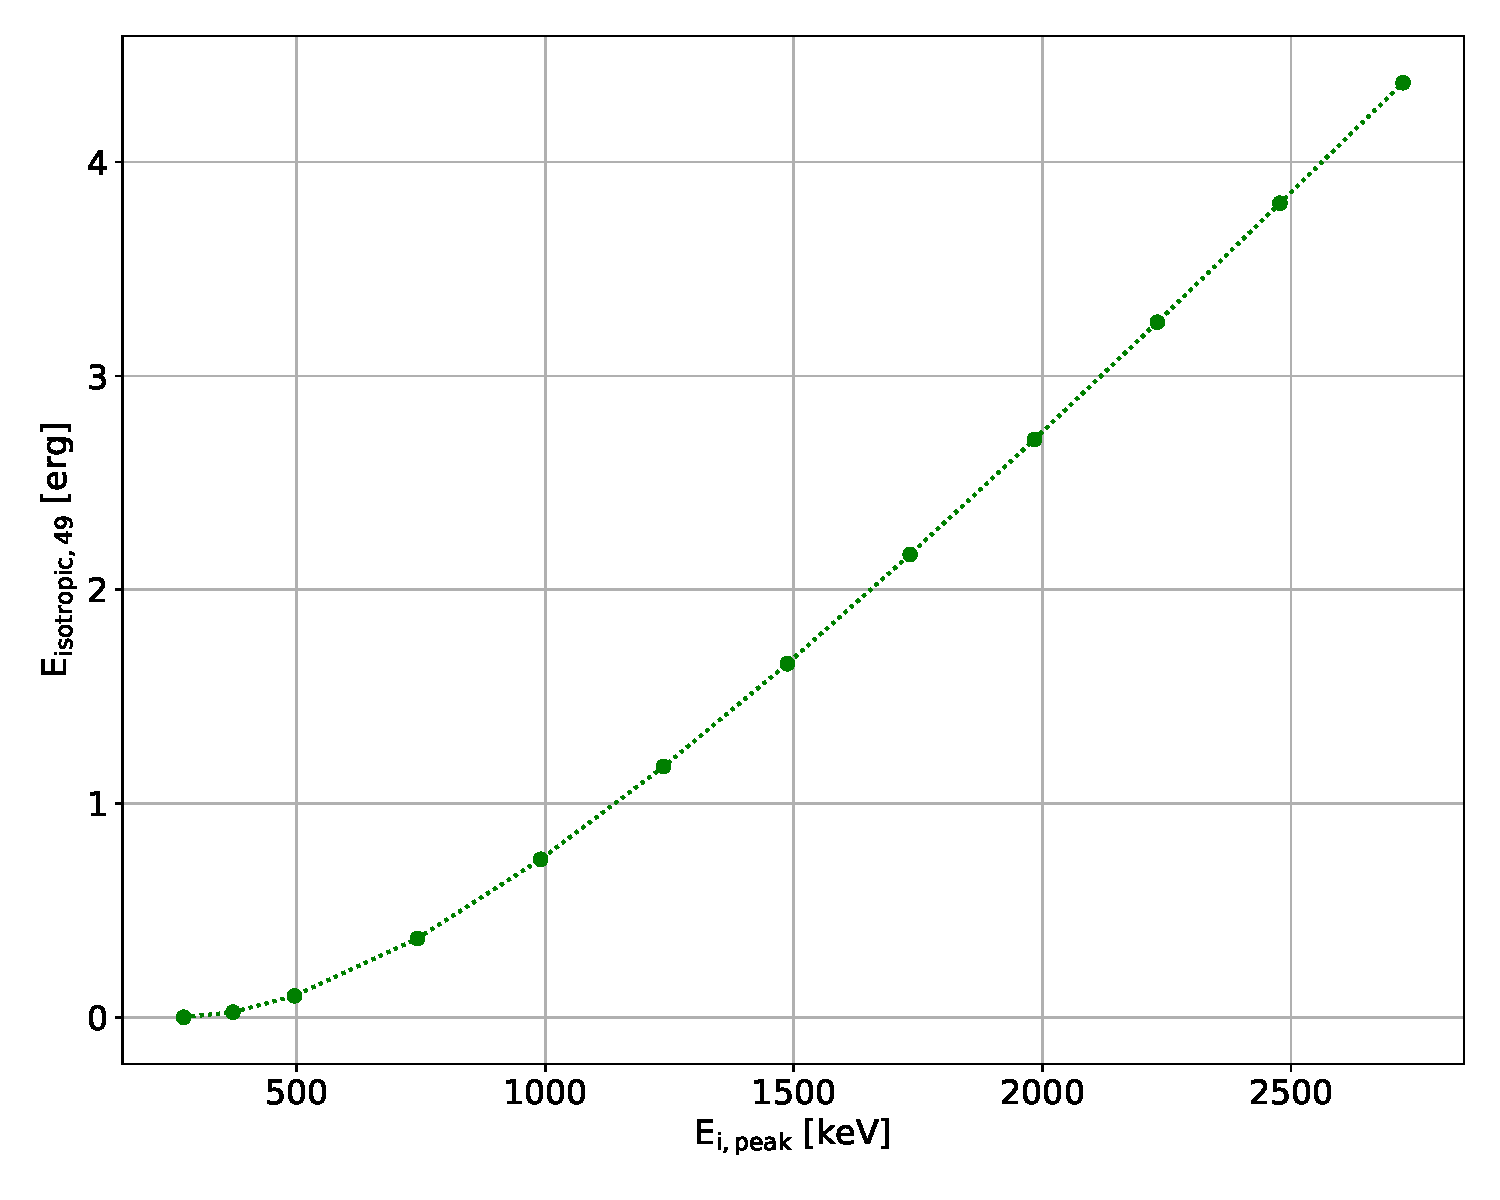
\includegraphics[width=\textwidth]{../ep3/Ep3__eipeak_eisotropic}%
%		\captionof{figure}{}
	\end{minipage}%

\newpage
%%%%%%%%%%%%%%%%%%%%%%%%%%%%%%%%%%%%%%%%%%%%%%%%%%%%%%%%%%%%%%%%%%%%%%%%%%%%%%%%%%%%%%%%%%%%%%%%%%%%
	\section{Combined time-integrated and time-resolved analysis}
	\begin{figure}[!h]
		\centering
		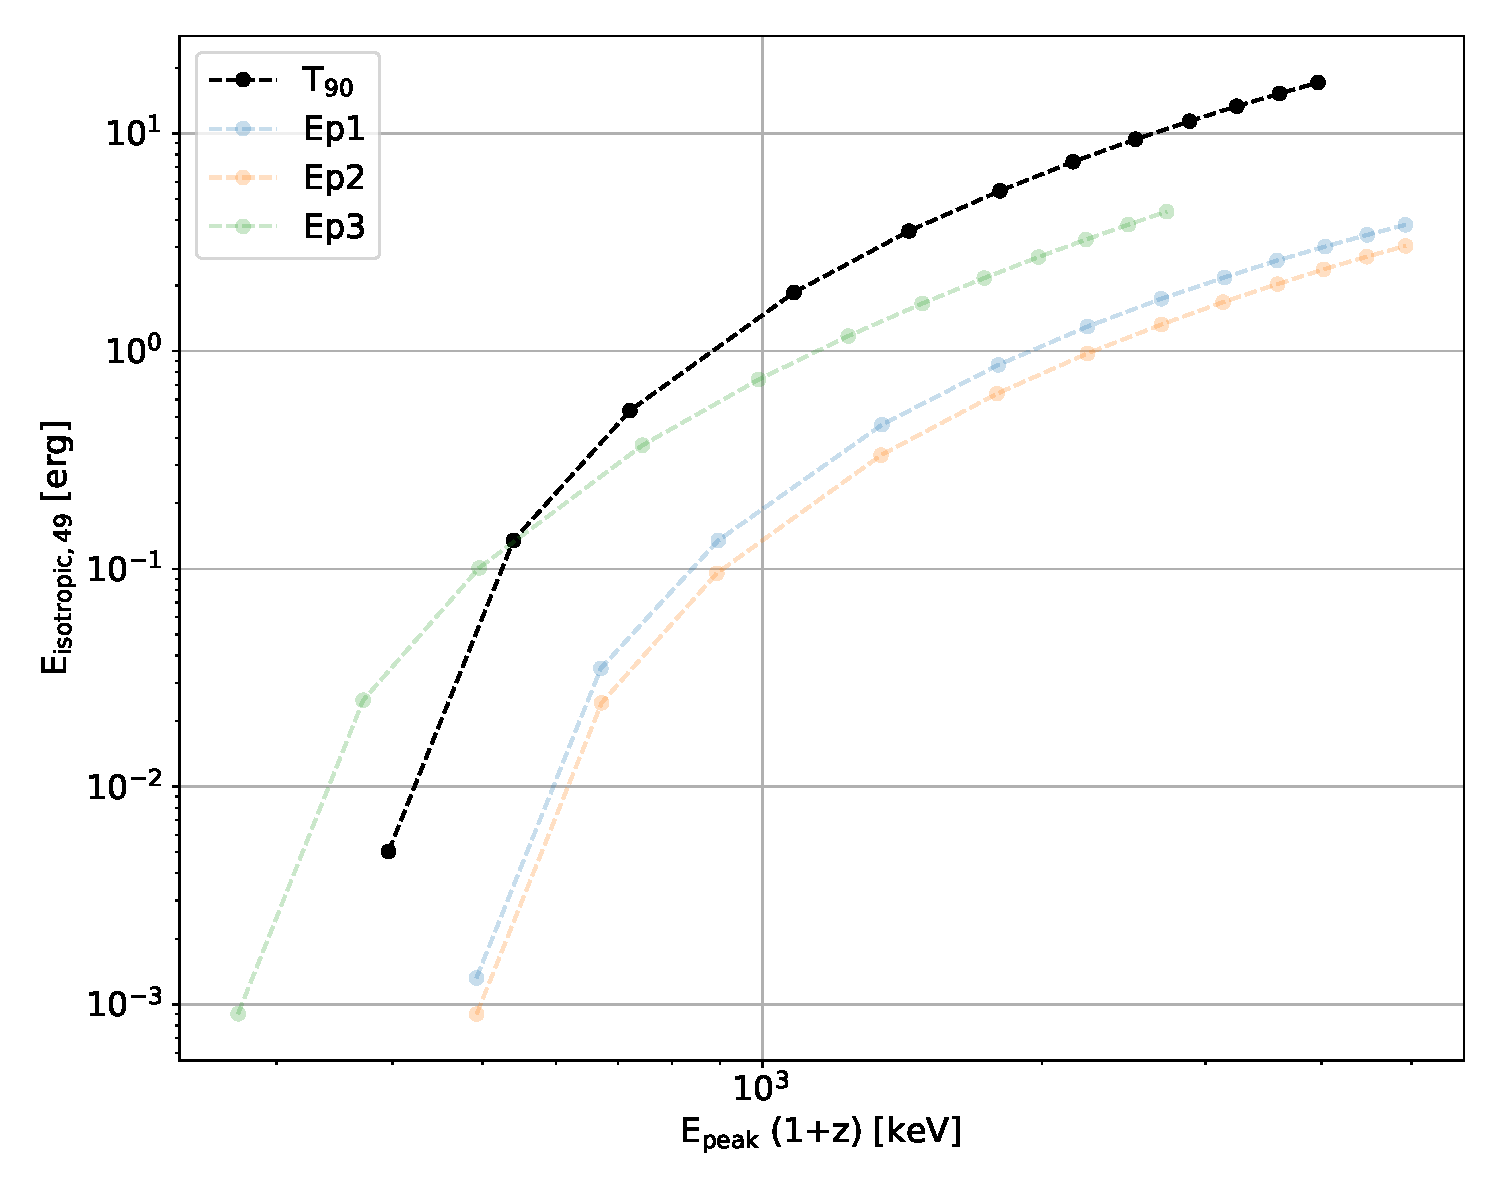
\includegraphics[width=\textwidth]{eisoep_compare}
		\caption{Combined E$_\text{isotropic}$ vs E$_\text{peak}(1+z)$ evolution.}
		\label{fig:eisoepcompare}
	\end{figure}
	

%%%%%%%%%%%%%%%%%%%%%%%%%%%%%%%%%%%%%%%%%%%%%%%%%%%%%%%%%%%%%%%%%%%%%%%%%%%%%%%%%%%%%%%%%%%%%%%%%%%%

	\section{Summary}
	The redshift corrected peak energy value for the first emission episode is fractionally more than the second one. This is despite the fact that the duration of first emission episode is only \SI{3.776}{\second}, whereas that of the second emission episode is \SI{4.8}{\second}. Although the third emission episode does not have a higher redshift corrected peak energy value, it does show the maximum isotropic energy out of the three emission episodes. Figure \ref{fig:eisoepcompare} shows the comparison between the E$_\text{isotropic}-$E$_\text{peak}$ relationship for both the time-integrated and time-resolved analysis of GRB120709A.
		
	The light curves of the GRB120709A (see figure \ref{fig:lcdiscontinuousepsextra}) also show higher GBM emission in the second episode compared to the first one. However, we do have higher LAT emission in the first episode which can be the cause of peak energy shift towards higher energy levels. As for the third episode, even though it has the highest count rate in \SIrange{10}{400}{\kilo\electronvolt}, it has next to negligible count rate in all other energy ranges. 
	\begin{figure}[!h]
		\centering%
		\includegraphics[width=\textwidth]{../../LCs/0_064/lc_discontinuous_eps__extra}%
		\captionof{figure}{Light curves for GRB120709A.}
		\label{fig:lcdiscontinuousepsextra}%
	\end{figure}
	

\end{document}